%        File: test.tex
%     Created: Thu Apr 21 03:00 PM 2011 C
% Last Change: Thu Apr 21 03:00 PM 2011 C
%

\documentclass[a4paper]{article}

\usepackage{amsmath}
\usepackage{graphicx}

\begin{document}

\section{Problem}
We have sampled a set of $m$ individuals $I$ from the general population. For each individual $i \in I$ we have gathered some information:
\begin{itemize}
  \item A matrix $V$ of size $m \times l$ that contains the set of sampled SNPs for each individual. Each element $s_{i,j} \in \{0,1,2\}$ describes the number of alleles for SNP $j$ for individual $i$.
  \item A matrix $R$ of risk factors of size $n \times k$. Each element $r_{i,j} \in \{0,1\}$ describes the risk factor $j$ for individual $i$.
  \item A vector $c$ of length $n$ that classifies each individual $i$ as healthy ($c_i = 0$) or sick ($c_i = 1$).
\end{itemize}
The problem is to find risk factors that are good predictors of the disease.

\section{Method}
The core idea is to find a set of axis aligned hyperplanes that maximizes the area under the resulting ROC curve.
\begin{itemize}
  \item Values $v_{i,l}$ (e.g. an individual SNP and risk factors) where $i \in [m]$ and $l \in [k]$.
  \item Classification $c_i$ where $i \in [m]$.
\end{itemize}

We will set up this as a quadratic programming problem. Let us first define a variable $n_{i,l}$ that determines whether individual $i$ was chosen when considering dimension $l$ (DESCRIPTION). Below is a list of conditions for the quadratic programming problem:

\begin{itemize}
  \item $0 \leq n_{i_1,l} \leq \dots \leq n_{i_m,l} \leq 1$ where $i_1, \dots, i_m$ is a permutation such that $v_{i_1,l} \leq \dots \leq v_{i_m,l}$. This conditions says that the values in dimension $l$ will be split into two connected parts, and also that each $n_{i,l}$ must be between $0$ and $1$ (hopefully either $0$ or $1$).
  \item Let $n_{i,l} \leq n_{i,l'}$ where $l' \in [l]$. This says that if $v_{i,j}$ was chosen in some dimension $l' \leq l$ then it must also be chosen in $l$.
\end{itemize}

The ROC curve is determined by a set of values $x_l$ which is the fraction of false positives when having defined hyperplanes for dimensions $1$ to $l$, $y_l$ is the fraction of true positives when having defined hyperplanes for dimensions $1$ to $l$. The area under the ROC curve can then be calculated by:
$$ AUC(n) = \frac{1}{2} \sum_{l=0}^{k+1} (x_l(n) - x_{l-1}(n))(y_l(n) + y_{l-1}(n)) $$
where $x_0(n) = y_0(n) = 0$ and $x_{l+1}(n) = y_{l+1}(n) = 1$. The functions $x_l(n)$ and $y_l(n)$ are in turn defined as:
$$ x_l(n) = \sum_{i=1}^{m} x_{i,l}(n), \qquad y_l(n) = \sum_{i=1}^{m} y_{i,l}(n)$$

The function $x_{i,l}(n)$ is $1$ for a false postive and $0$ otherwise, similarly $y_{i,l(n)}$ is $1$ for a true postive and $0$ otherwise. The variables $x_{i,l}(n)$ and $y_{i,l}(n)$ then relates to $n_{i,l}$ as follows:
$$x_{i,l}(n) = n_{i,l}(1-c_i)$$
i.e. if $n_{i,l}$ is chosen ($=1$) then $x_{i,l}(n)$ is $1$ only when individual $i$ is healthy.

\section{Problems with this approach}
If two of the sampled values have a AND relationship, for example if a disease is dependent on having a specific SNP, AND a high blood preasure, we cannot find it using the approach above. If we think back to the discrete case, each assignment of the risk factors was added in the order of their slope in the ROC curve. But in the continuous case we construct the ROC curve by adding a half plane in one dimension at a time. The proper generalization would be to add one cell at a time in the grid generated by the hyperplanes.

\begin{figure}[h]
  \centering
  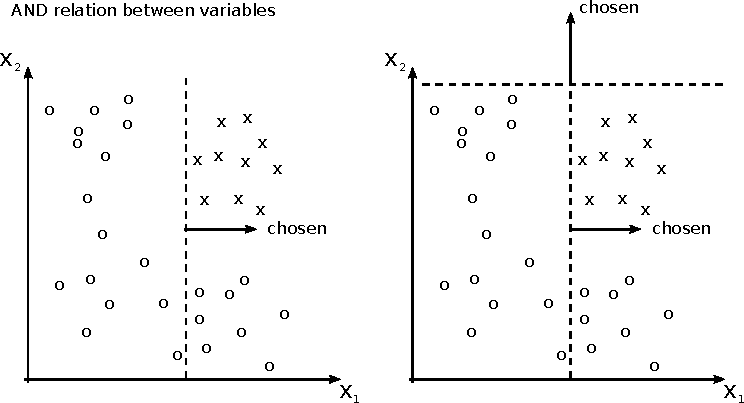
\includegraphics[scale=0.8]{graphics/problem}
  \caption{Illustrates how the hyperplanes becomes illpositioned if two variables have an AND relationship.}\label{fig:problem}
\end{figure}
\end{document}
